We conducted surveys on Amazon Mechanical Turk~\cite{mturk} to judge the quality of colors and palettes generated by \system. The study evaluated the following hypotheses:

\textbf{H1:} Machine-generated colors are perceived to be more topic-relevant than colors chosen randomly a standard palette.
\textbf{H2:} Machine-generated palettes are perceived to be more likable and aesthetically pleasing than palettes of colors randomly chosen from a standard palette. 

\subsection{Method}
To test \textbf{H1} (\textit{topic relevance}), we showed 50 participants from Mechanical Turk six options for each topic. Four of them were colors generated by \system. One was a random color picked from the Protovis palette, which is also used by several other visualization programs. The last choice was none of the above. Participants picked the one choice that they felt best suited the topic.

To test \textbf{H2} (\textit{palette likability}), we tried four objective functions for generating a palette. One tried to pick the most frequent color, another optimized for saturation, one maximized perceptual distance between the colors. The last objective picked colors from the topic at random (so there was no maximization, but distance constraints were satisfied). We asked 49 participants from Mechanical Turk to rate our four variations and one randomly generated palette, from Protovis on a scale of 1-7.

We drew topics the topics tested in both studies from six different categories. We classified these categories as being either concrete or abstract. Concrete categories involved tangible objects: football teams, sodas, and fruits. Abstract categories involved ideas or concepts that do not have a concrete manifestation: emotions, academic disciplines, and countries. 

\subsection{Results}
\subsubsection{Topic Relevance} 
We found that the \system colors were preferred significantly over the random Protovis colors and none of the above ($\chi^2$(2, N=50) = 83.76, $p <$ 0.001). 947 times out of 1200, Turkers picked a \system color.  Thus, \system is able to pick at a set of colors for a topic that contains at least some appropriate colors.

\begin{figure}
\label{relevance}
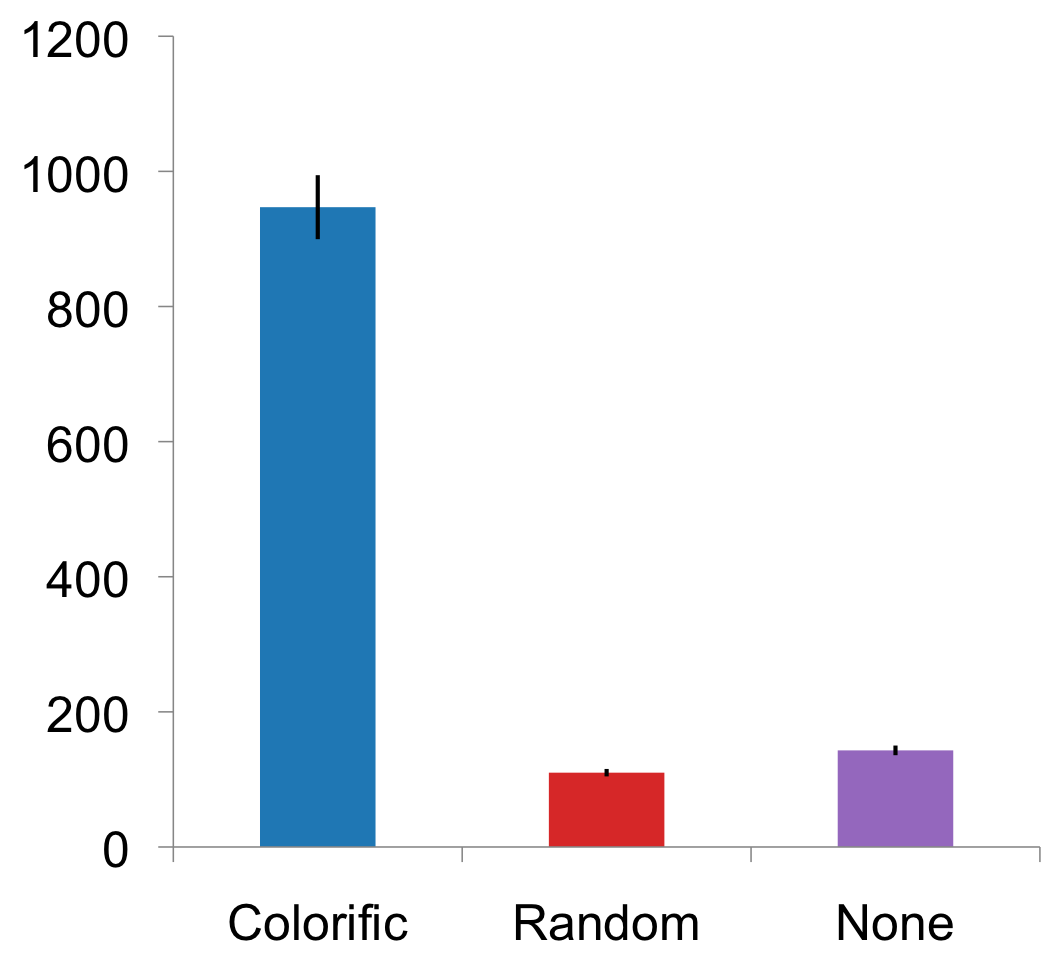
\includegraphics{relevance_chart.png}
\caption{Participant preferences for single color. \system colors outperformed Random and None.}
\end{figure}

\subsubsection{Palette Likability by Algorithm} 
A Friedman test revealed a significant effect of the type of algorithm used to generate the palettes on rating ($\chi^2$(4)=15.40, $p <$ 0.005). A post-hoc test using Wilcoxon signed-rank tests showed the significant differences between frequency and Protovis palettes ($p <$ 0.05, r = -0.117) and between distance and Protovis palettes ($p <$ 0.05, r = -0.142).

\subsubsection{Palette Likability by Category}
A Friedman test revealed a significant effect of the palette category on rating ($\chi^2$(5)=37.51, $p <$ 0.001). However, no significant difference was present between our concrete and abstract categories. Although some palette categories significantly perform better than others, our concrete/abstract classification failed to capture why.

\begin{figure}
\label{likability}
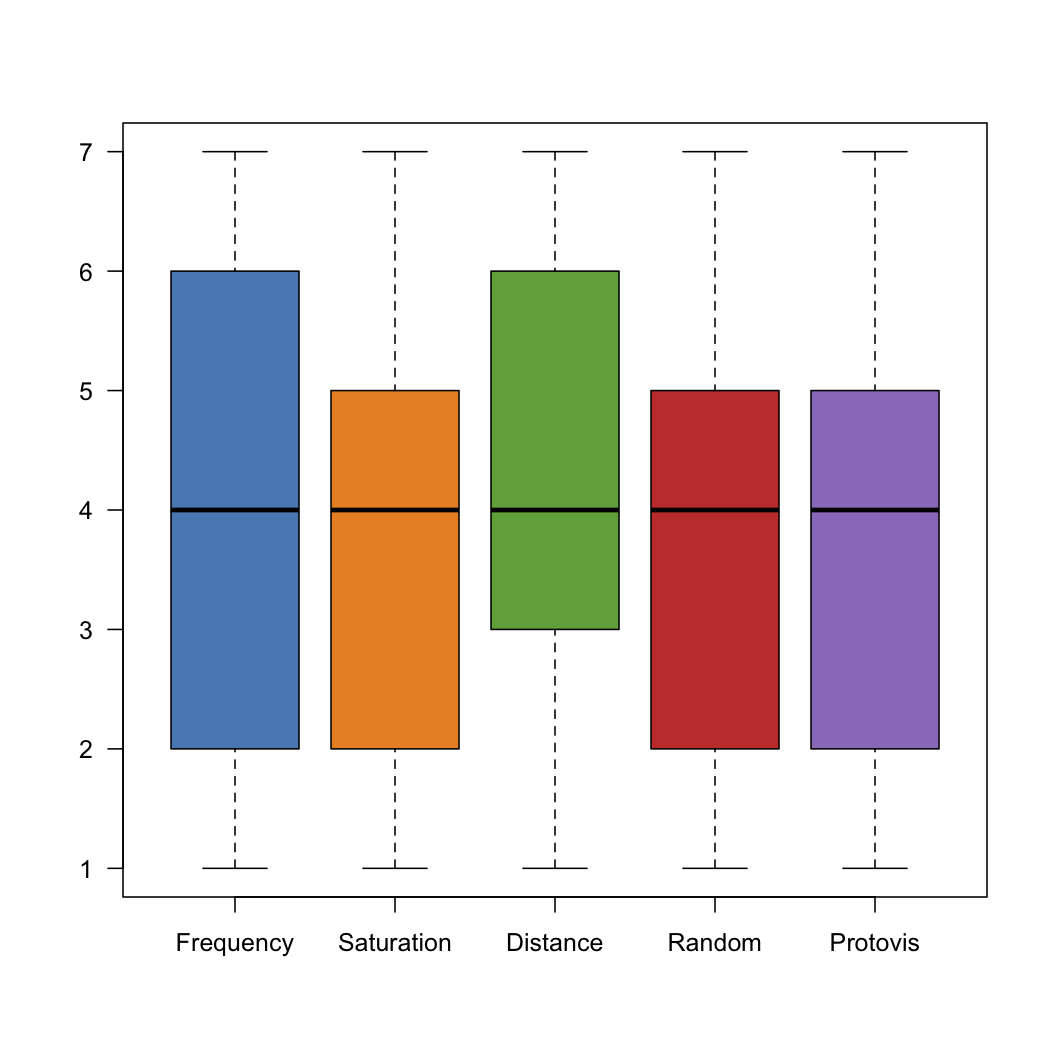
\includegraphics{likability_algorithm.png}
\caption{Participant ratings on a scale of 1-7 (7: most likable) for color palettes}
\end{figure}